\chapter{Estudios, optimizaciones y mejoras} \label{cap:analisis}
Llegados a este punto nos planteamos realizar varios estudios relativos al rendimiento del algoritmo evolutivo, basadas en inquietudes fundadas en numerosos artículos científicos, para verificar que no se estaba produciendo ninguna inconsistencia dentro del entrenamiento de dicho algoritmo evolutivo. Además, también realizamos una serie de optimizaciones sobre funciones ya existentes en JECO, con el fin de reducir lo máximo posible el tiempo de ejecución y retocar algunas opciones por defecto del framework evolutivo para mejorar los resultados.

\section{Estudio de la presión selectiva}
Una de los factores que consideramos de importancia dentro de nuestro algoritmo evolutivo es la conservación de diversidad dentro de nuestra población y tratar de evitar el estancamiento en óptimos locales, la convergencia prematura y la evolución en avalancha producidas por la falta de ésta diversidad. Para ello hemos decidido evaluar cuál es la presión selectiva durante la ejecución, siendo esta la frecuencia con que es seleccionado el mejor individuo frente al resto. Esto se calcula en problemas de maximización mediante la siguiente fórmula
\begin{equation*}
\textrm{Presión selectiva} = \frac{\textrm{fitness mejor}}{\textrm{fitness promedio}}
\end{equation*}
En nuestro caso, al ser el nuestro un problema de minimización ($100000 - score$) empleamos:
\begin{equation*}
\textrm{Presión selectiva} = \frac{\textrm{fitness promedio}}{\textrm{fitness mejor}}
\end{equation*}

Habitualmente se recomienda emplear una presión selectiva en torno a $1.5$ \cite{whitley1989genitor}, mientras que nosotros a partir de mediciones hemos comprobado que empleamos una de aproximadamente $1.35$. Además, cada vez que se produce una mejora del mejor \textit{fitness}  se produce un aumento proporcional en la presión selectiva, volviéndose a equilibrar al adaptarse el \textit{fitness} promedio a esta mejora. No obstante, dicho aumento de la presión selectiva es despreciable.
 
Concluimos que tenemos una presión selectiva adecuada y por tanto no requerimos la implementación de ningún sistema de escalado del \textit{fitness} de los individuos para mantener una conservación de diversidad.
\begin{figure}[H]
\centering
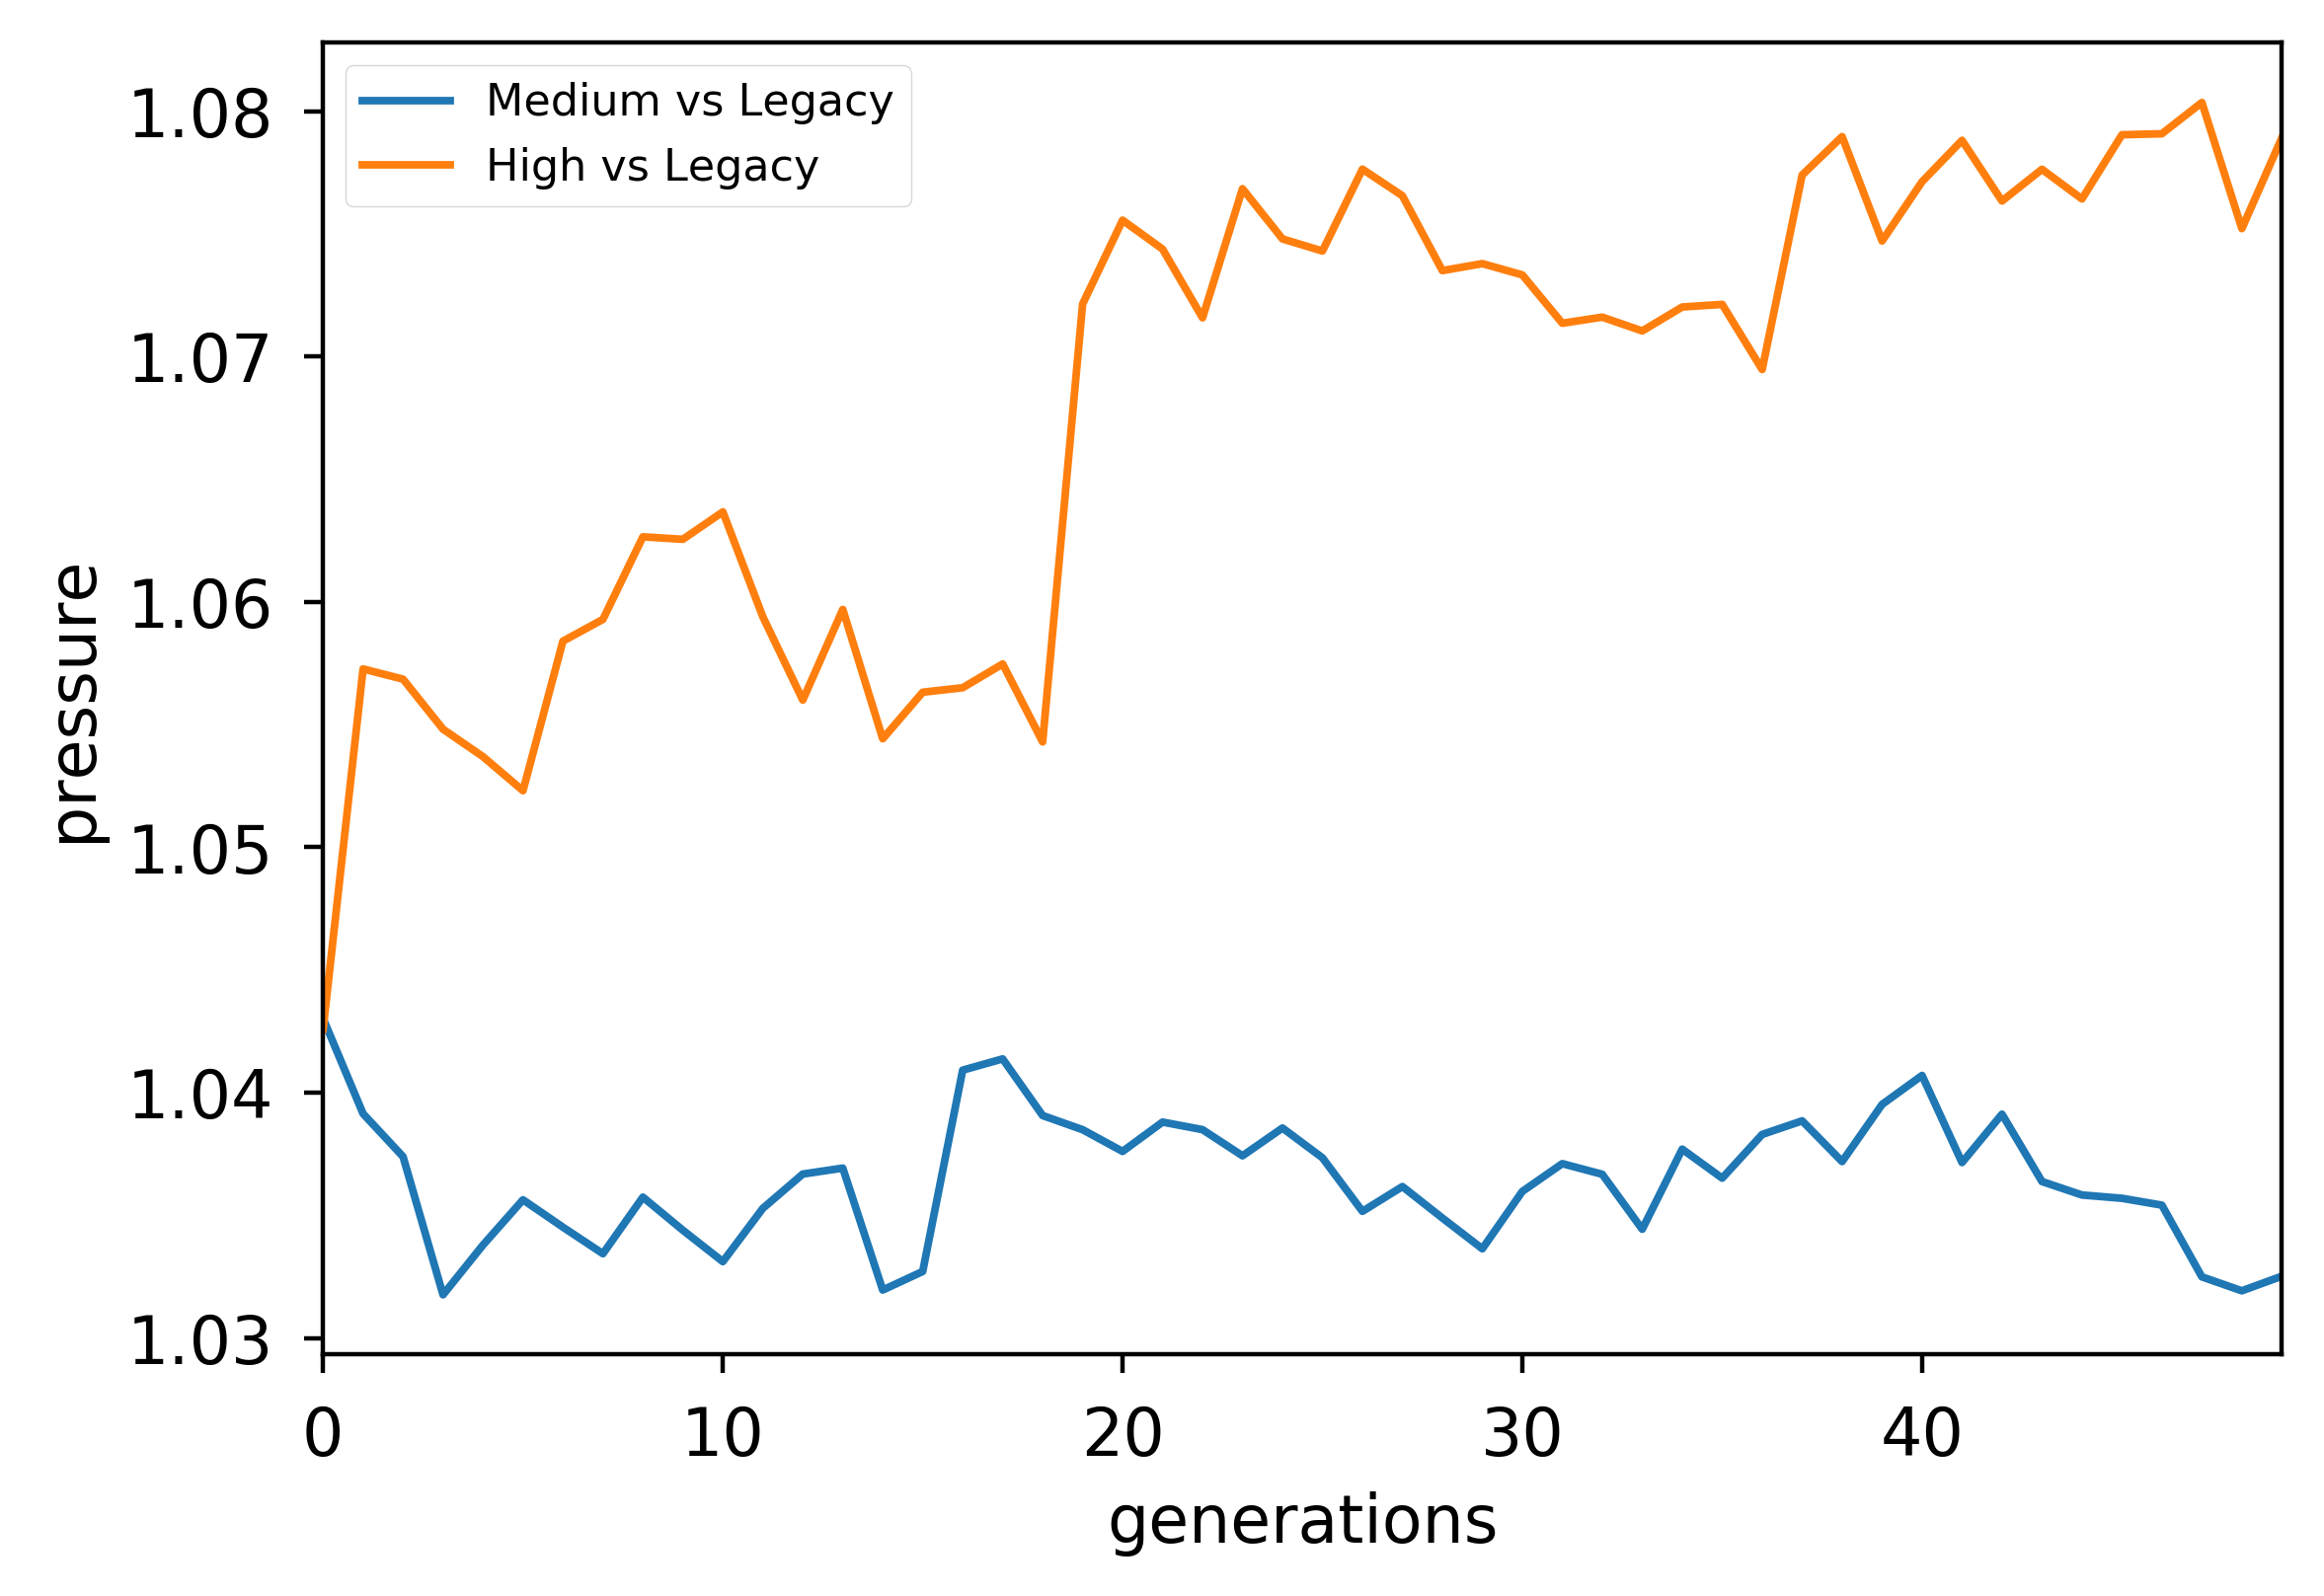
\includegraphics[width=0.8\textwidth]{grafica/presion-selectiva-detalle}
\caption{Vista en detalle  de la presión selectiva.}
\end{figure}

\begin{figure}[H]
\centering
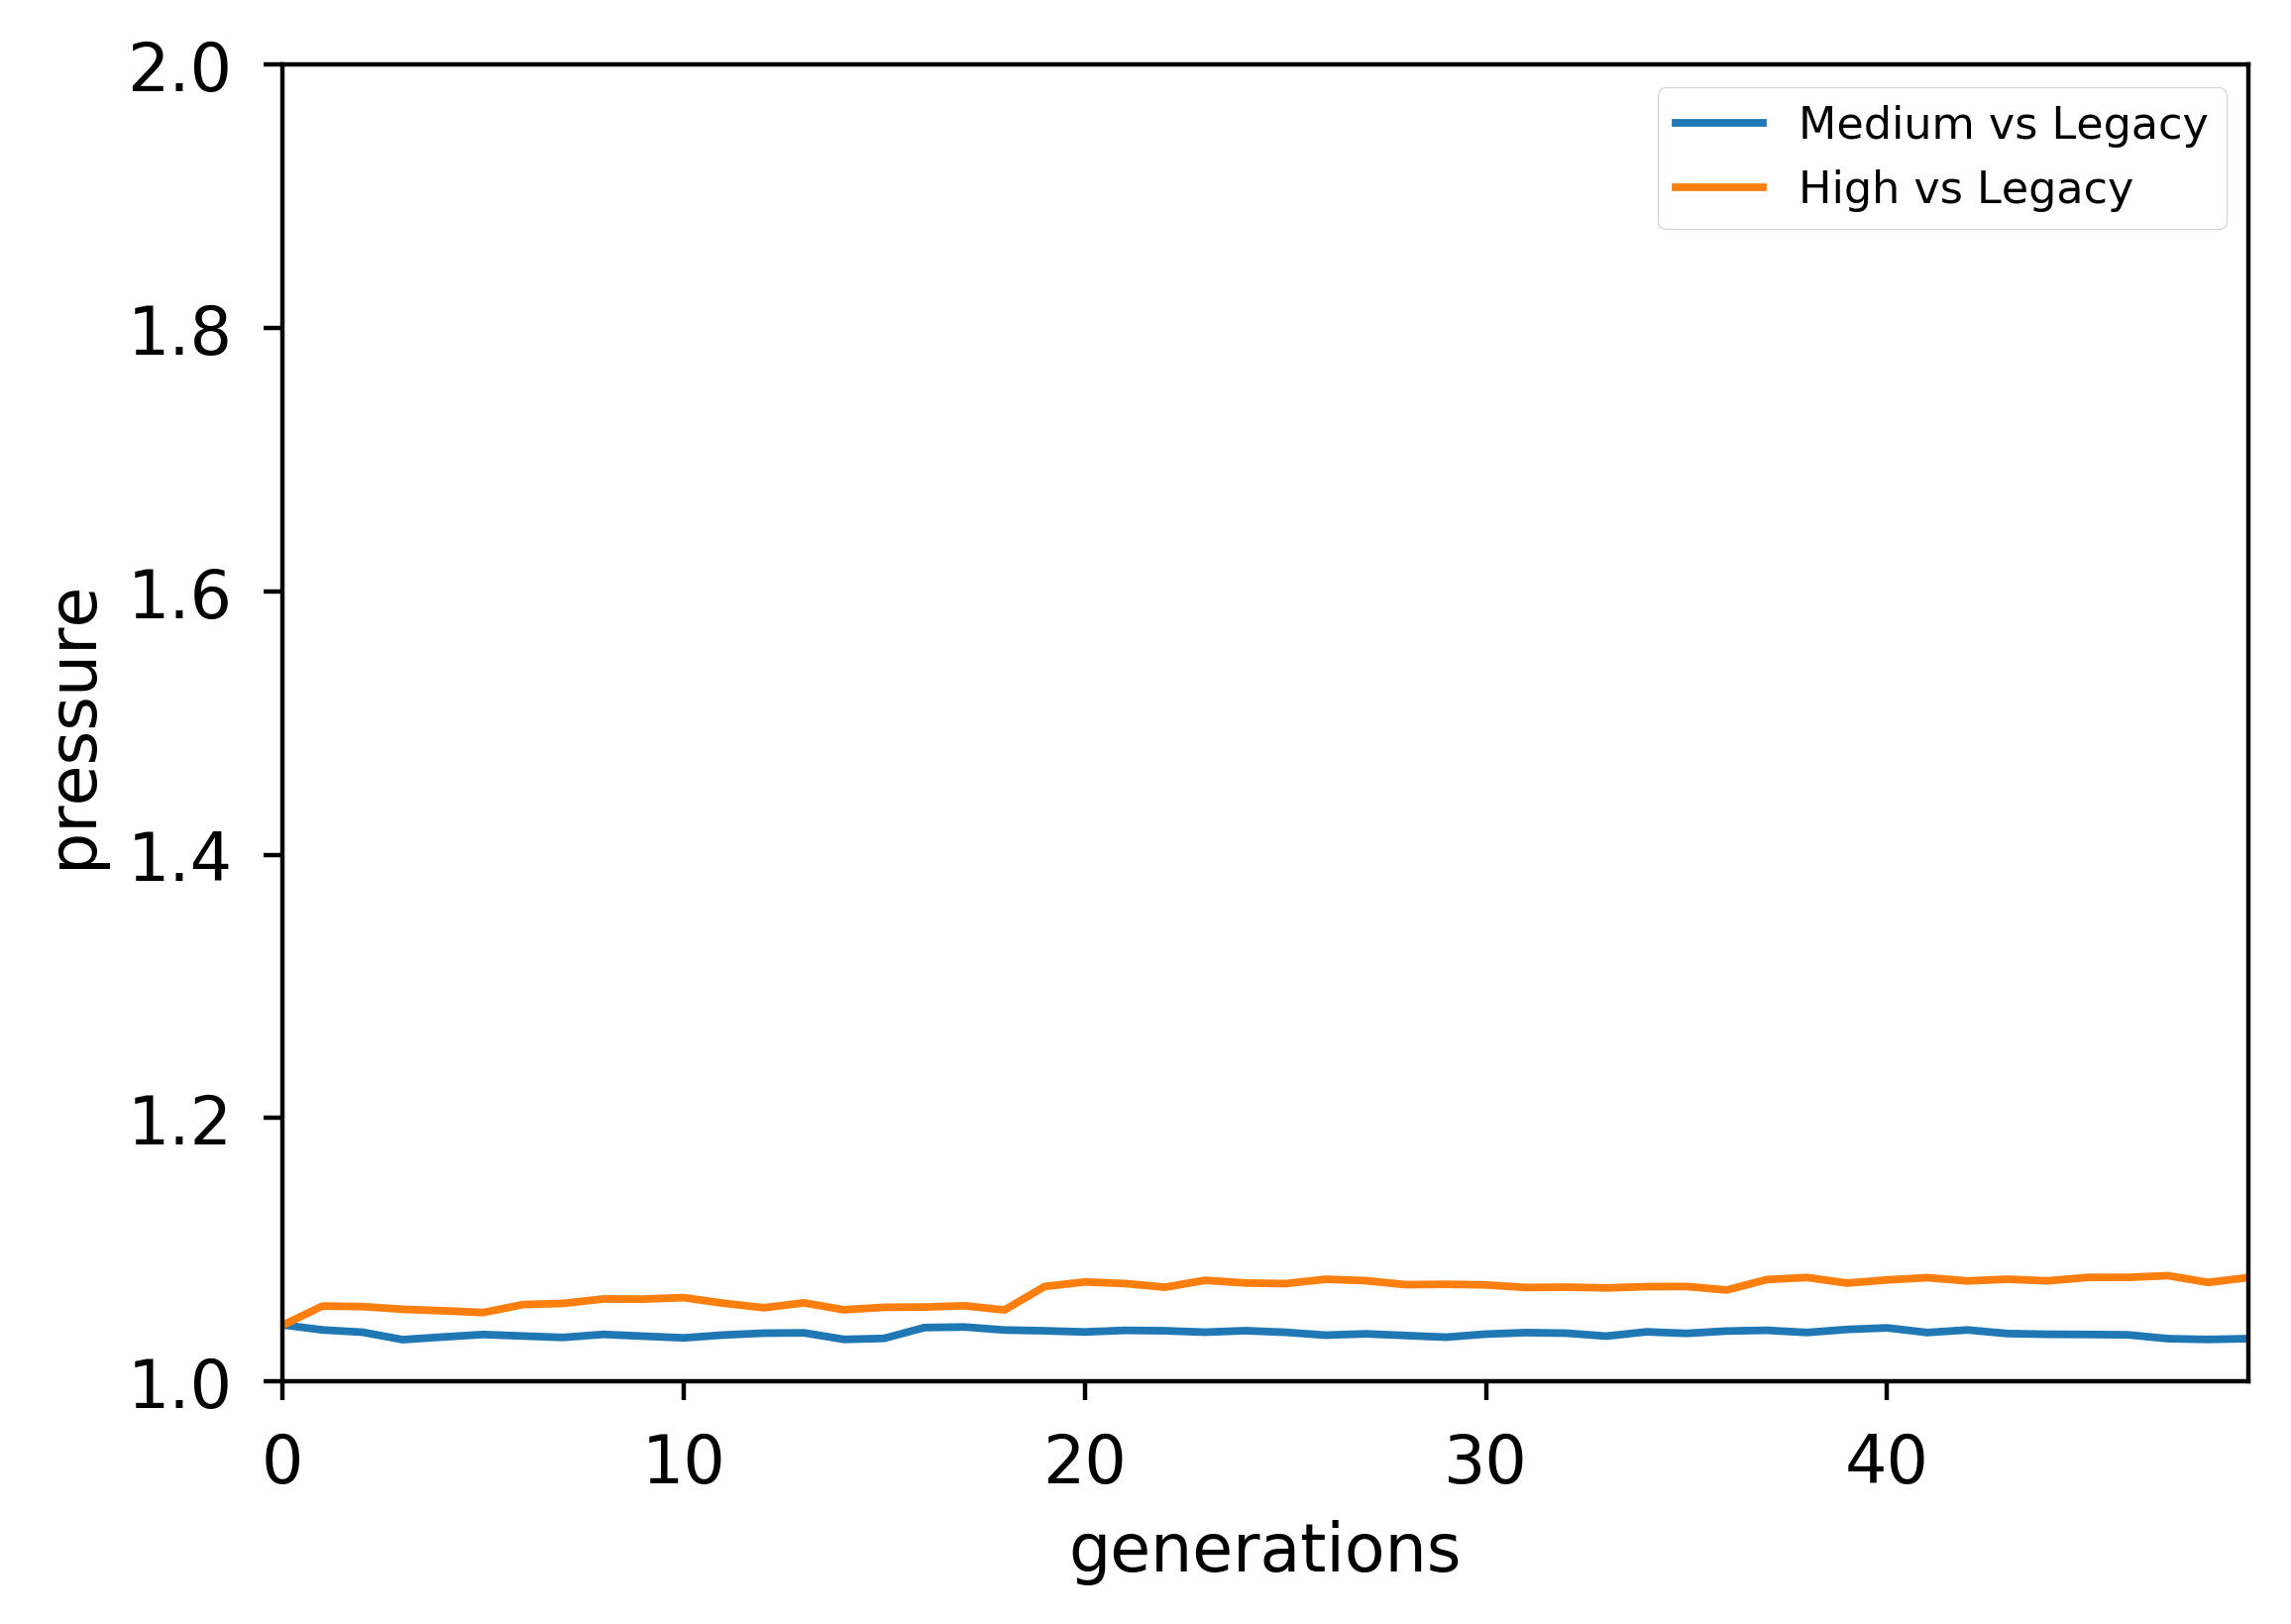
\includegraphics[width=0.8\textwidth]{grafica/presion-selectiva-general}
\caption{Vista global de la presión selectiva.}
\end{figure}

Además, tras un estudio en profundidad de nuestros operadores de selección hemos comprobado que todos (Torneo Binario, Torneo Binario NSGA y Torneo n-ario) emplean alguna modificación del operador de torneo, siendo este independiente al valor de la presión selectiva. Esto es así porque estos operadores no tienen en cuenta comparaciones entre fitness relativos (por ejemplo seleccionar proporcionalmente más veces los individuos con mejor fitness) sino comparaciones directas (seleccionar el individuo con mejor fitness entre varios elegidos de forma completamente aleatoria).

\section{Cruce LHS}
Antes de proceder con el estudio de nuevas funciones de \textit{fitness} decidimos comprobar si la razón por la que se producían programas tan cortos en las gramáticas de medio y alto nivel era por culpa del operador de cruce utilizado.

El operador de cruce monopunto usado en Gramáticas Evolutivas tiene el problema de generar mucho ruido en la población porque al cruzar los dos genotipos el nuevo hijo no suele guardar ninguna relación con los padres dada la forma en que se genera el fenotipo. Visto de otra forma, el cruce no copia un trozo de código de un individuo en el código del otro individuo, sino que lo altera desestructuradamente.

Para resolver este problema se implementa el cruce LHS que intenta solventar este problema. El cruce LHS, al igual que el monopunto, elige un punto aleatorio del genotipo pero en vez de cruzar la parte del genotipo restante a partir de ese punto lo que hace es ver cuántos codones expanden el símbolo no terminal marcado por el punto de cruce. Una vez visto cuántos codones componen la derivación total de dicho símbolo estos se insertan en la posición del punto de corte en el otro individuo, donde también se ha realizado el mismo proceso.

Este nuevo cruce produce ligeramente mejores resultados y menos ruido en la población pero tampoco se aprecia una gran mejoría en general. Aún así se convierte en el principal cruce que utilizamos en adelante.

\section{Estudio de uso de codones}
Durante la implementación del cruce LHS hicimos un estudio del número de codones utilizado en cada individuo para generar el fenotipo. El estudio lo hacemos con individuos de 100 y 50 codones permitiendo hacer \textit{wrapping}\footnote{El Wrapping se produce cuando se han procesado todos los codones del genotipo y aún no se ha llegado a procesar todos los símbolos no terminales dejando el fenotipo incompleto por lo que se sigue expandiendo los símbolos sin procesar usando nuevamente los codones del principio del genotipo.} 3 veces.  Los resultados obtenidos son los siguientes:
\begin{figure}[H]
\centering
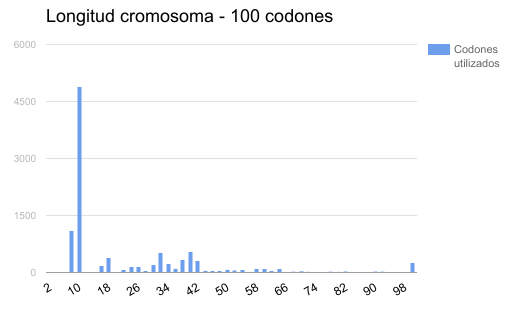
\includegraphics[width=0.8\textwidth]{grafica/codones-100}
\caption{Distribución del número real de codones utilizados. Longitud máxima 100 codones.}
\end{figure}

\begin{table}[H]
\centering
\begin{tabular}{|c|c|c|c|c|}
\hline
\textbf{Media} & \textbf{Wrappings} & \textbf{Moda} & \textbf{Mediana} & \textbf{Desviación  est.} \\ \hline
23.9           & 331                & 10            & 10               & 21.7                      \\ \hline
\end{tabular}
\caption{Estadísticas con longitud del cromosoma = 100.}
\end{table}

\begin{figure}[H]
\centering
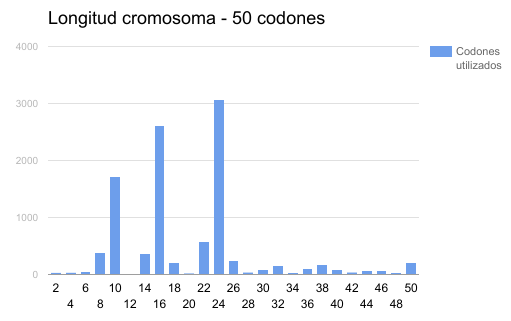
\includegraphics[width=0.8\textwidth]{grafica/codones-50}
\caption{Distribución del número real de codones utilizados. Longitud máxima 50 codones.}
\end{figure}

\begin{table}[H]
\centering
\begin{tabular}{|c|c|c|c|c|}
\hline
\textbf{Media} & \textbf{Wrappings} & \textbf{Moda} & \textbf{Mediana} & \textbf{Desviación  est.} \\ \hline
20           & 375                & 24            & 18               & 9                      \\ \hline
\end{tabular}
\caption{Estadísticas con longitud del cromosoma = 50.}
\end{table}

Como se puede ver, cuando se usan longitudes de 100 codones los fenotipos se generan en su mayoría usando solo diez codones, lo que implica programas muy cortos y que la mayoría de las mutaciones y cruces sobre ellos no tienen efecto dado que se producen en el 90\% de los codones del genotipo que no se usan.

En cambio, con una longitud de 50 codones los individuos suelen generar individuos más largos, usando 25, 16 y 10 codones normalmente. Lo que sugiere que longitudes más pequeñas de cromosomas implican programas más largos a los que una mutación o un cruce los afecta en mayor medida y que pueden llegar a generar mejores resultados.

Para comprobar esto realizamos un banco de pruebas donde comprobar si es verdad que longitudes de cromosomas más cortas producen mejores resultados. Evolucionamos varias poblaciones idénticas pero variando en cada una la longitud de sus cromosomas, usando valores de 10 a 100 incrementados de diez en diez.

Los resultados obtenidos de este banco de pruebas no aportaron nada dado que los resultados y longitudes de fenotipos en las poblaciones con longitudes entre 40 y 100 eran prácticamente iguales, por lo que concluimos que la longitud del cromosoma no tiene mucha relación con los resultados obtenidos.

\section{Estudio de funciones fitness}
Como ya hemos visto, las gramáticas de bajo y medio nivel producen comportamientos demasiado específicos e incluso indeseados pero que consiguen muchos puntos. Hemos decidido probar nuevas funciones y ver el comportamiento obtenido por el bot. Para estas pruebas utilizaremos la última versión de la  gramática de nivel medio y con los mismos valores y operadores para los operadores de cruce, mutación, etc (Apartado~\ref{sec:params}).
\begin{itemize}
\item \textit{Puntuación \{1000000 - puntuación media\}}: Es la función de \textit{fitness} que se utiliza de forma genérica. Puntúa a los individuos por la puntuación media obtenida al evaluarlos, siendo los mejores individuos aquellos que obtengan mayor puntuación media.

Esta función se estanca siempre en un óptimo local produciendo el bot ``cazador'' el cual solo busca comerse el mayor número de fantasmas dado que esta acción produce una gran cantidad de puntos, pero una vez acabadas las \textit{power pill} realiza movimientos neutrales o come la \textit{pill} más cercana sin importarle la posición de los fantasmas, por lo que es eliminado por los fantasmas y no es habitual que complete el nivel uno.

\begin{lstlisting}[caption={Mejor individuo obtenido mediante esta función fitness.}]
    if( getDistanceToClosestEdibleGhost <= 20 ){ 
        getDirectionTowardsClosestPowerPill
    }
\end{lstlisting}

\item \textit{Pills \{1000 - media de pills consumidas\}}: \textit{Fitness} que tiene como objetivo comer el máximo número de \textit{pills} posibles, sin importar la puntuación obtenida ni el nivel, aunque este último está directamente relacionado con comer \textit{pills}. Al mejor individuo que suele producir le hemos denominado bot ``Glotón''.

Este bot se centra únicamente en comer \textit{pills} normales pero, si se siente amenazado por un fantasma cercano, se dirige hacia una \textit{power pill}, la consume y sigue comiendo \textit{pills} normales (pero no caza a los fantasmas). Cuando no dispone de más \textit{power pills} a las que dirigirse y un fantasma se acerca, este sigue comiendo \textit{pills} normales y es comido por los fantasmas. Este bot suele perder en el nivel dos o en el nivel uno cuando quedan pocas \textit{pills} por comer. El código producido es el antónimo del producido por el \textit{fitness} de \textit{Puntuación}.

\begin{lstlisting}[caption={Mejor individuo obtenido mediante esta función fitness.}]
    if( getDistanceToClosestNonEdibleGhost >= 25 ){ 
        getDirectionTowardsClosestPill
    }
    else{ 
        getDirectionTowardsClosestPowerPill
    }
\end{lstlisting}

\item \textit{Niveles \{10 - máximo nivel alcanzado\}}: El objetivo de este \textit{fitness} es pasarse el mayor número de niveles sin importar la puntuación, las \textit{pills} comidas, el tiempo utilizado, etc por lo que los mejores individuos son los que han llegado al nivel más avanzado. Este bot nos sorprendió dado que aprovecha el fallo del juego que provoca que no sea detectado por algunos controladores de fantasmas como \textit{Starter ghosts}, si se coloca en una cierta posición del laberinto.

Este ``exploit'' lo conocíamos pero nunca se había producido en el nivel tres, sin embargo este bot consigue realizarlo en todos los niveles llegando a superar\footnote{La versión actual del juego soporta un número ilimitado de niveles pero dispones de un tiempo máximo de juego (24000 \textit{ticks}). El juego es detenido si se consume el tiempo total, independientemente del nivel en el que te encuentres. Dado que la versión actual del juego hace que se avance de nivel automáticamente al estar 4000 \textit{ticks} en el mismo nivel el número máximo de niveles al que se puede llegar usando el fallo del juego (estancándose en una parte del laberinto sin moverse hasta que se avanza de nivel por tiempo) es de $24000 / 4000 = 6$ niveles.} el juego. Se trata del bot ``Camper'' pero con un comportamiento mejorado. Nos dimos cuenta de que este comportamiento es alcanzable con las funciones \texttt{getDistanceToClosestJunction\{Up, Down, Right, Left\}}. Si eliminamos dichas funciones de la gramática de medio nivel entonces se produce un bot ``Camper'' que no supera el nivel cuatro.
\end{itemize}

Observamos que el bot se especializa dependiendo del objetivo de la función \textit{fitness} como es de esperar. No obstante contra controladores de fantasmas especialmente bien diseñados como \textit{Legacy} la diversidad de comportamientos decrece, ya que en Pac-Man la mayoría de objetivos están relacionados (por ejemplo, para pasarse niveles Pac-Man ha de comerse todas las \textit{pills} si le es imposible ``atascar'' a los fantasmas y ganar el nivel por agotar el tiempo).

En cualquier caso decidimos explorar una estrategia multiobjetivo con la intención de conseguir un comportamiento acorde a lo que se debería esperar de un jugador \textit{amateur}, avanzar el máximo número de niveles consiguiendo la mayor cantidad posible de puntos, comportamiento que no conseguimos usando una función \textit{fitness} con un único objetivo en consideración contra todos los tipos de fantasmas.

\section{Optimización Multiobjetivo}
Para intentar solventar el problema de especialización que se está produciendo contra algunos tipos de fantasmas decidimos implementar una estrategia multiobjetivo en el algoritmo.

Existen varios métodos de implementación de estrategias multiobjetivo y por la primera que nos decantamos fue una estrategia mediante funciones agregativas. Decidimos usar esta estrategia en primer lugar porque no altera el algoritmo de gramáticas evolutivas que estamos usando actualmente. Consiste en la implementación de una función \textit{fitness} (como hasta ahora) pero que consta de una combinación lineal de funciones o parámetros que cada una determina la valía de un individuo en un determinado aspecto.

\subsection{Funciones Agregativas}
La primera función agregativa mediante este método fue la unión de las anteriores funciones fitness de comer el máximo número de pills y alcanzar el mayor nivel. La unión directa de las funciones como una combinación lineal del estilo
\begin{equation*}
f = \textrm{nº de pills} + \textrm{nivel máximo alcanzado}
\end{equation*}
no es posible por la diferencia de escala de los objetivos (el número de \textit{pill} comidas va a ser siempre más grande que el nivel máximo alcanzado por lo que ese objetivo no tiene impacto visible en el \textit{fitness} del individuo) por lo que el uso de unos pesos $w_i$ serán necesarios para que ambas funciones tengan la misma importancia en la combinación lineal.

Dada la función
\begin{equation*}
f = w_0 * \textrm{nº de pills} + w_1 * \textrm{nivel máximo alcanzado}
\end{equation*}
tuvimos que experimentar varias versiones con distintos valores de los pesos wihasta conseguir un balance adecuado. La versión final de la función fue
\begin{equation*}
f = \textrm{nº de pills} + 10 * \textrm{nivel máximo alcanzado}
\end{equation*}
donde $w_0 = 0$ y $w_1 = 10$.

Los resultados no fueron los esperados y normalmente se obtenía un comportamiento de bot ``Glotón'' en los mejores casos pero se vio un incremento en la longitud media de los programas (fenotipo) evolucionados.

El mismo proceso se realizó con la unión de las funciones \textit{fitness} de conseguir puntos y avanzar de niveles
\begin{equation*}
f = 0.1 * \textrm{nº de puntos obtenidos} + \textrm{nivel máximo alcanzado}
\end{equation*}
donde $w_0 = 0.1$ y $w_1 = 1$ pero se obtuvo un bot ``Camper'' pero con un código menos eficiente y llegando hasta el cuarto nivel de media.

\begin{lstlisting}[caption={Código del bot Camper obtenido mediante funciones agregativas.}]
if( getDistanceToClosestJunctionLeft >= 60 ){ 
    getDirectionTowardsClosestPill
 }
 else{ 
    if( getDistanceToClosestEdibleGhostUp > 75 ){ 
        if( getClosestEdibleGhostDistanceToClosestJunctionLeft < 30 ){ 
            if( getDistanceToClosestNonEdibleGhost <= 50 ){ 
                getDirectionTowardsClosestEdibleGhost
             }
             else{ 
                getDirectionTowardsClosestEdibleGhost
             }
         }
         else{ 
            if( getDistanceToClosestNonEdibleGhost <= 10 ){ 
                if( getClosestEdibleGhostDistanceToClosestJunctionDown <= 5 ){ 
                    getDirectionAwayFromClosestNonEdibleGhost
                 }
                 else{ 
                    getDirectionTowardsClosestPowerPill
                 }
             }
 
         }
     }
     else{ 
        getDirectionTowardsClosestPill
     }
 }
\end{lstlisting}

Nuevamente no obtenemos los resultados esperados y el proceso de creación de combinaciones lineales es experimental, poco preciso y tedioso, así que nos decidimos a realizar una implementación avanzada de la estrategia multiobjetivo mediante el uso del algoritmo NSGA-II el cual usa la definición de óptimo de Pareto y frente de Pareto en su algoritmo para determinar los mejores individuos en los objetivos a optimizar.

\subsection{NSGA-II}
JECO disponía de una implementación del algoritmo NSGA-II que nos sirvió como base para desarrollar la implementación de la estrategia multiobjetivo mediante NSGA-II. Los cambios realizados en JECO a nivel de código se explicarán en el apartado~\ref{sec:multi}).
 
Hemos desarrollado una serie de funciones fitness por cada objetivo que deseemos optimizar. Hemos intentado representar los objetivos típicos que un jugador humano amateur intenta conseguir.

\paragraph{Naive fitness}
Puntuación directa obtenida en juego, en la que se tienen en cuenta \textit{pills}, \textit{power pills} y fantasmas comidos. Cuantos más puntos mejor \textit{fitness} obtenido (minimización).
\begin{equation*}
f = 1000000 - \textrm{puntuación media}
\end{equation*}

\paragraph{Ghosts eaten}
Número de fantasmas comidos. Cuantos más fantasmas consumidos mejor fitness tendrá el individuo.
\begin{equation*}
f = 1000 - \textrm{fantasmas comidos}
\end{equation*}

\paragraph{Levels completed}
Número de niveles completados. A mayor nivel alcanzado mejo fitness del individuo.
\begin{equation*}
f = 100 - \textrm{último nivel alcanzado}
\end{equation*}

\paragraph{Points without ghost multiplier}
La puntuación total obtenida pero sin emplear el multiplicador de puntos que utiliza Pac-Man al comer varios fantasmas seguidos.
\begin{equation*}
\begin{split}
f = 100000 - (\textrm{número de pills consumidas} * \textrm{puntos por pill consumida}) \\
+ (\textrm{número de power pills consumidas} * \textrm{puntos por power pill consumida}) \\
+ (\textrm{número de fantasmas consumidos * puntos por fantasma consumida})
\end{split}
\end{equation*}

\subsection{Resultados}
Desafortunadamente, la inclusión de multiobjetivo no parece marcar una diferencia notable. Si por ejemplo usamos los \textit{fitness} \textit{Naive} y \textit{Levels completed} no se obtienen mejores bots que los mismos \textit{fitness} por separado. Esto se debe a que los objetivos que se pueden crear para el juego dependen directa o indirectamente de la puntuación, por lo que no se crea diversidad de comportamiento en nuestros programas. Lo que nos lleva a pensar que funcionaría mucho mejor cuando los objetivos no están directamente relacionados.
 
Los resultados muestran que si forzamos el objetivo de alcanzar más niveles, los programas obtenidos alcanzan puntuaciones similares ya que Pac-Man avanza niveles comiendo todas las \textit{pills} del laberinto, y por tanto consiguiento puntuaciones más altas. Lo mismo pasa al contrario, si nos centramos en conseguir puntos, Pac-Man completará todos los niveles que le sea posible porque se centra en comerse todas las \textit{pills}.
 
De cualquier forma siempre tenemos una ventaja clara usando multiobjetivo; en vez de definir un comportamiento monolítico podemos crear un diseño más modular, más fácilmente, añadiendo subobjetivos adicionales a los ya escogidos. Como por ejemplo comer \textit{pills} y mantenerse lo más alejado posible de los fantasmas, lo que le hace sobrevivir más tiempo.

\section{Mutación neutral}
La Mutación Neutral es un operador específico para gramáticas evolutivas \cite{oesch2015neutral} que pretende proporcionar más diversidad a la población realizando una mutación que no afecta al fenotipo. Esto es posible en gramáticas evolutivas, ya que si modificamos un codón del fenotipo de un individuo sumándole un múltiplo del número de producciones de la regla que determinó esa parte del fenotipo, el fenotipo resultante es el mismo. Por ejemplo, si tenemos un símbolo no terminal expandible a través de cuatro reglas de producción a los codones mutados se les suma a su valor actual un múltiplo de cuatro (dado que hay cuatro reglas de producción) por lo que al generar el fenotipo y realizar el módulo al codón este devolverá el mismo número que antes de la mutación, produciendo el mismo fenotipo.

Aunque se mantiene el mismo fenotipo del individuo, se gana una mayor diversidad, ya que en evaluaciones posteriores el genotipo de este individuo ha podido ser modificado a través del operador de cruce o un operador de mutación adicional que sí produzca cambios (como Mutación bit a bit) y este cambio en el codón ya no tiene por qué producir el mismo módulo y modificará el fenotipo.

Un ejemplo de mutación neutral podría ser el siguiente:

\begin{lstlisting}[caption=Gramática e individuo de ejemplo para aplicar mutación neutral]
<S> ::= <B> | <C> | <D>
<B> ::= b | a
<C> ::= c | a
<D> ::= d | a 
\end{lstlisting}

Codones del individuo: \texttt{8 6 4 3 7 5 \dots}

Primero usaríamos el codón $8$ para expandir \texttt{S}. El número de producciones posibles para \texttt{S} es $3$. Así pues, haríamos $8 \mod 3 = 2$, optaríamos por expandir usando \texttt{D}.
Lo interesante es que para $11$, $14$, $17$, y en definitiva la suma de $3$ al codón el número de veces que queramos, obtenemos el mismo resultado. Por lo tanto podemos hacer la siguiente suma al valor del codón:

\begin{equation*}
\textrm{codón} = \textrm{codón} + (n * \textrm{número producciones posibles para el no terminal a expandir})
\end{equation*}

donde $n$ es un valor entero arbitrario mayor que $1$. Así se mantiene la selección de producciones intacta (y por lo tanto el fenotipo del individuo, el árbol), mientras que el genotipo (el propio codón) sí varía.

El mismo proceso se realizaría ahora para ver si expandimos \texttt{D} con \texttt{d} o \texttt{a}, y lo mismo vuelve a ser aplicable, permitiéndonos en definitiva mutar todos los codones utilizados del individuo con garantía de no modificar su fenotipo.

\section{Multithread}
Al empezar a desarrollar el segundo bot también pudimos aprovechar otra funcionalidad de JECO que consiste en paralelizar la etapa más pesada del algoritmo (evaluación) en los distintos procesadores del ordenador.

Así, las etapas donde se ejecutan los operadores de selección, cruce y mutación se hacen en el mismo hilo de procesamiento, ya que estas etapas son más llevaderas, con algún operador ejecutándose por ejemplo un 10\% de las veces en la iteración. Y seguidamente cuando llegamos a la etapa de evaluación, podemos dividir la tarea entre tanto núcleos como haya disponibles para ejecutar el juego 1, 10, 20 o incluso más veces para paliar la aleatoriedad de los fantasmas, y eso para cada individuo de la población.

Gracias a esta técnica nos hemos podido permitir poblaciones más grandes y mayor número de generaciones en las evoluciones sin que los tiempos para completarlas sean desorbitados.


\section{Optimizaciones secundarias de JECO}
El framework JECO nos es de mucha ayuda, pero ha habido ciertos momentos en los que se necesitaban ciertos ajustes o carecía de ciertas funcionalidades que nos hacían falta, por lo que las hemos tenido que implementar a mano. Las más importantes son:

\subsection{Creación de las clases para cada función fitness}
Se implementó un patrón de diseño \textit{Command} para estructurar la creación de funciones de \textit{fitness}. Así todas las funciones, aunque dispares, tienen un punto común que funciona de acuerdo a lo esperado.

\subsection{Wrapper de funciones fitness para su uso en multiobjetivo} \label{sec:multi}
Gracias al patrón \textit{Command} para las clases de las funciones de fitness se pudo implementar una factoría de clases fitness y un envoltorio (\textit{FitnessWrapper}). A esta clase se le pasan las funciones creadas fácilmente desde \textit{ObjectiveFactory} cuando se quieren cambiar objetivos, incluso en tiempo de ejecución. Después, \textit{FitnessWrapper} es llamado cada vez que se evalúa el algoritmo en las sucesivas generaciones, justo después de ejecutar Pac-Man para pasarle las estadísticas de la partida.

\subsection{Modificación de la mutación}
La mutación por defecto en JECO se realiza únicamente sobre los individuos que son resultantes de un cruce. Mezclar cruce y mutación de esta manera no nos ha dado buenos resultados, y lo hemos sustituido por una aproximación más común en los Algoritmos Genéticos: Primero se aplica el operador de cruce a los elementos seleccionados de la población anterior, y después se aplica el operador de mutación a toda esa nueva población de elementos seleccionados e hijos generados por el operador de cruce. De esta manera garantizamos la independencia de operadores, ya que de lo contrario, tener una probabilidad de cruce muy baja implicaba que el operador de mutación se aplicase con una probabilidad distinta y solo a ciertos elementos.

\subsection{Modificación de la élite}
JECO utiliza un método particular a la hora de mantener la élite en la población. En cada generación y después de haber realizado la selección, cruce y mutación en los individuos pertinentes JECO unía la población antigua y la nueva población, constituida por los elementos seleccionados y los hijos creados a través de aplicar el operador de cruce, creando una unión de poblaciones ordenada de mejor a peor fitness. De este nuevo conjunto se extrae el número de individuos máximo que pueden haber en una población.

Este método no aporta diversidad a la población dado que se usa toda la población de la anterior generación (sin alterar) y la nueva población para generar la población final que será utilizada en la siguiente generación, haciendo que muchos individuos de la anterior generación se conserven en la nueva generación (y normalmente a lo largo de muchas generaciones más) conduciendo la búsqueda rápidamente a un óptimo local del cual es difícil de salir por falta de diversidad.

Optamos por deshacernos de esta implementación e implementamos un elitismo clásico, donde un subconjunto de los mejores individuos de la población antigua (determinado por un parámetro denominado porcentaje de elitismo) se incluyesen en la nueva generación sustituyendo un porcentaje idéntico de peores individuos en la nueva población, aportando mayor diversidad y permitiendo que la búsqueda no se estanque tan rápido en un óptimo local e incluso pudiendo salir de él.
\begin{figure}[H]
\centering
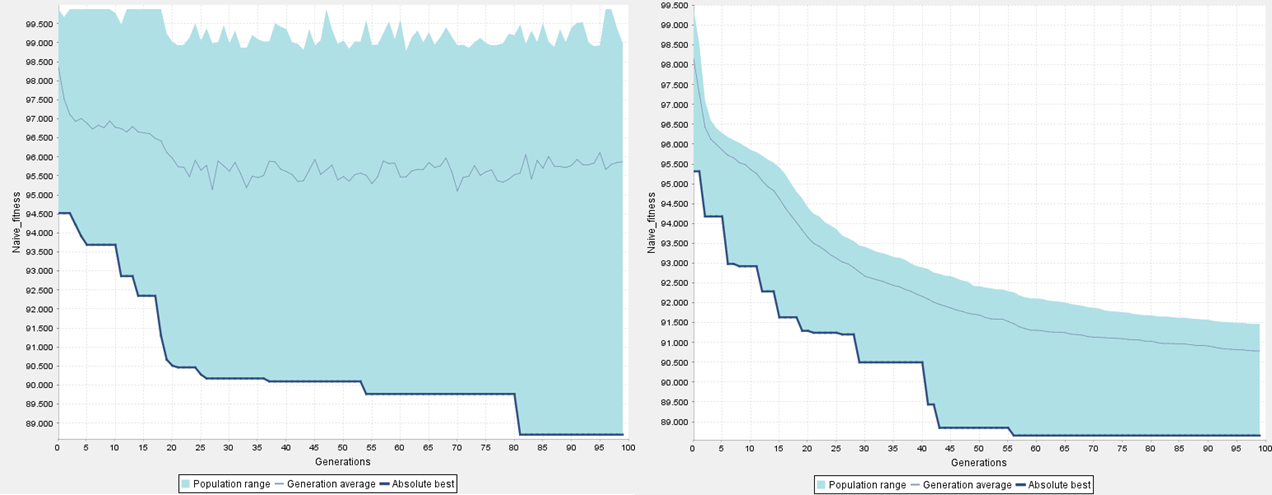
\includegraphics[width=\textwidth]{comparacion-elite}
\caption{A la izquierda gráfica de la evolución de la población con el nuevo método de elitismo. A la derecha gráfica usando el método de elitismo de JECO usado anteriormente. La línea gris muestra la media del fitness de la población.}
\end{figure}

\section{Batch Executor}
Debido que empleamos controladores de fantasmas no deterministas, necesitamos ejecutar varias partidas con un mismo controlador de Pac-Man para obtener resultados estadísticamente correctos de su rendimiento. Puesto que aumentar el número de partidas que juega un mismo individuo en la evaluación del algoritmo evolutivo supone un impacto significativo en el tiempo de ejecución de este, optamos por ejecutar un número conservador de partidas (unas 30, como queda reflejado en el parámetro iterspeind de la tabla con los mejores parametros \ref{table:best-params}).
 
Una vez terminada la ejecución del algoritmo evolutivo, extraemos el código del mejor individuo producido. Después empleamos este código para jugar mil partidas contra el controlador de fantasma deseado.
 
Gracias a este procedimiento podemos obtener datos precisos manteniendo tiempos de entrenamiento razonables. Requerimos esta reevaluación mas precisa del bot debido a la gran aleatoriedad del comportamiento de controladores de los fantasmas. Cabe destacar el hecho de que a partir de 1000 partidas no se produce ninguna mejora en la precisión de los datos obtenidos.
